\documentclass{article}

\usepackage{float,amsthm,amsmath,amssymb,amsthm,graphicx,enumerate,hyperref}
\usepackage{fancyvrb}
\graphicspath{ {./images/} }

\usepackage{pgfgantt}
\usepackage{lscape}

\usepackage{xcolor}
\hypersetup{
	colorlinks,
	linkcolor=black,
	citecolor=black,
	urlcolor=black
}

\begin{document}
	\begin{titlepage}
	\vbox to \textheight{
	\begin{center}
		\begin{figure}[H]
			\centering
			
\includegraphics[width=0.3\textwidth]{logo.jpeg}
			\\[25pt]
		\end{figure}
		\begin{Large}
			\textbf{B.Sc. (Special) Degree in Computer Science \\ University of Sri Jayewardenepura} 
		\end{Large}
		\\[50pt]
		\begin{large}
			\textbf{An Independent Research Proposal\\}
		\end{large}
		\vspace{2cm}
		\begin{Large}
			\textbf{A companion robot for employees in a company to increase productivity by reducing their stress level}\\
		\end{Large}
		\vspace{1cm}
		K.G.S.Sandaruwan\\
		AS2016502\\
		\vspace{3cm}
		Academic Year 2020\\
		Supervisor: Dr. Ravindra De Silva
	\end{center}
	\vfill}
\end{titlepage}
	
	\tableofcontents
	\newpage

	\section{Introduction}
	Most people in the society should be employed so that they are able to earn enough (money) to live and provide for themselves and their family. Although naturally, these may include meals, clothes and sanitary wear; a person also needs other items, a few luxury items every now and then, a fancy dress for a wedding or a new phone, to feel content and satisfied with life, so as not to feel worthless.\\
	
	\indent According to the ``International Standards Classification of Occupations\cite{iscoDefinition}'', there are 10 categories of occupations in the world. From that list, the people who are working in the 4 top-most of those categories are mostly doing their jobs using the mental power rather than their physical power. When dividing those 4 categories into more sub-categories, about half of them are indoor occupations. That means people who are doing these jobs are usually sitting on a chair with a table, working with stationary or sitting in front of a computer.\\
	
	\indent Working in the same and consistent environment for a long time tends to make most people bored of that environment\cite{workingEnvironmentBoredom} and it leads to reduction in productivity of that person and hence the company too. This may happen at any place that is very steady and even. As mentioned above, a person who sits on a chair in front of a computer or books for a long time may face this problem frequently. Not only for an employee in an office, but a child in a study room also may face this problem frequently.\\
	
	\indent As mentioned earlier, most peoples work to earn to support their families. The majority of the workers are fathers\cite{genderDistribution} who on average have to provide for a family of four. Unless someone has a 6 figure salary, this could naturally be a stressful feat to any person, taking into fact that he is wholly and completely responsible for the living of another human being. Sometimes disagreements with these very individuals can be more distressing than any other factor. Especially for these reasons, missing these other individuals can also lead to feeling lonely and being less productive due to the poor mindset. However the same dependents could be the reason for them to work their best, being motivation to the employee.\\
	
	\indent I decided to find a solution for this problem, while narrowing down the scope into “Employee in an software development company” scenario. Here I decided to use a companion robot, that can identify stress level, drowsiness, loneliness and other uncomfortable feelings or moods of the employee by observing behavioral traits of that particular person, then analyzing them against time, and finally responding in such a way that it rids the employee from feeling lonely or drowsy and help them to have a stress free mindset which results in an improved level of productivity.
	
	\section{Significance of the Research}
	The major problem faced by most of people in the working environment is the workplace boredom due to feeling uncomfortable, followed by getting stressed. Non-physical discomfort highly affects a person, driving them towards boredom\cite{whyYouFeelBored} even if the working environment is physically comfortable. Loneliness and consistency have been identified as some of most frequent reasons for a lack of interest in the working environment which results to workplace boredom as mentioned above.\\ 
	
	\indent Everyone at their work are usually stressed in some level and sometimes it may be more than others. This could be bad for subordinators if the manager was feeling this way on that particular day. All the individuals could have a falling out, and have a bad mood for the rest of the day; or the work delegated could also be more than the worker thinks he is capable of and hence those individuals also may be stressed out making the situation worse.\\

	\indent So is there any way to do some small changes in the environment without disturbing that person's occupation related things, and to build up a feeling in those person, that he/ she is not isolated, or that he is not being singled out by the employee and not aggrieved from employer then those things may make that person comfortable in a non-physical way and therefore that employee may be inclined to work happier and agog\cite{happynessAndProductivity}. The workload that person can handle is quite higher than which is done when the person is in a bored and stressful mood.\\
	
	\indent So this robot may cause to improve the productivity of that particular person by reducing the boredom and stress of that employee, which in turn, improves the productivity of that company.
	
	\section{Research Objectives}
	\begin{itemize}
		\item Make the working environment look joyful from the employees’ perspective
		\item Increase the productivity of employees to develop the company from the employer’s perspective
		\item Increase the non-physical (mental) health of employees from the company's HR’s perspective
	\end{itemize}

	\section{Methodology}
	\subsection{Hardware Implementation(s)}
	\begin{itemize}
		\item Currently I have planed to build a small robot, that contains both interface and processing part in the same module, which can place on the employees' computer monitor. Then that robot will analyze facial muscles and eye movements of that employee.
		\item If some technical limitations occurred in university level, only the camera, display, speaker and such IO devices may embedded with interface module, which may placed on the monitor as mentioned above, and the module which stands for processing inputs and generating output signals may moved as an separated module, which is connected to interface part via a cables or Wi-Fi.
		\item Or else can make it a USB plugable device that do the processing part from that employee's machine itself with driver software and the interface module may be there same as the early case.
		\item To detect the uncomfortable situations of a human, I have to analyze raw data taken from camera, by processing those video frames. It may require some higher computation power to process those video frames. So a powerful micro-controller (likes Raspberry PIE) or an external computer (mini-pc) may be required for that. So not only the size and shape of hardware, the performance also should be considered.
		\item Actuators and motors to do movements which makes the employee happy
	\end{itemize}
	\subsection{Software Implementation(s)}
	\begin{itemize}
		\item Have to recognize the person who is currently sitting near the computer.
		\item If that person currently with some uncomfortable situations, then the system should detect those uncomfortable situations of that person.
		\item Decide the most suitable action to do according to the person's current situation.
		\item Command actuators and motors to perform the action decided.
	\end{itemize}
	
	\section{Design}
	\begin{figure}[H]
		\centering
		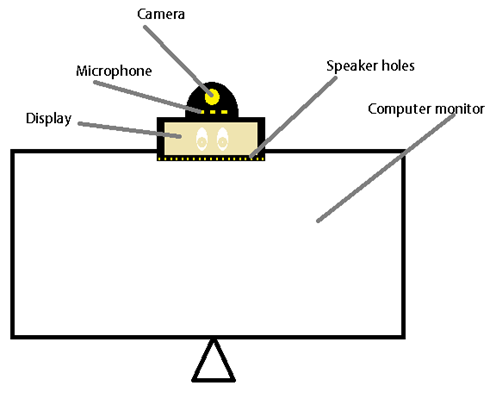
\includegraphics[width=1\textwidth]{design.png}
		\\[25pt]
	\end{figure}
	
	\section{Timeline}
	\begin{landscape}
		\definecolor{barblue}{RGB}{153,204,254}
\definecolor{groupblue}{RGB}{51,102,254}
\definecolor{linkred}{RGB}{165,0,33}
\renewcommand\sfdefault{phv}
\renewcommand\mddefault{mc}
\renewcommand\bfdefault{bc}
\setganttlinklabel{s-s}{START-TO-START}
\setganttlinklabel{f-s}{FINISH-TO-START}
\setganttlinklabel{f-f}{FINISH-TO-FINISH}
\sffamily

%\section*{\centering{Research Timeline}}

\begin{ganttchart}[
    canvas/.append style={fill=none, draw=black!5, line width=.75pt},
    hgrid style/.style={draw=black!5, line width=.75pt},
    vgrid={*1{draw=black!5, line width=.75pt}},
   ,
    % today label font=\small\bfseries,
    title/.style={draw=none, fill=none},
    title label font=\bfseries\footnotesize,
    title label node/.append style={below=7pt},
    include title in canvas=false,
    bar label font=\mdseries\small\color{black!70},
    bar label node/.append style={left=2cm},
    bar/.append style={draw=none, fill=barblue},
    bar incomplete/.append style={fill=black!18},
    bar progress label font=\mdseries\footnotesize\color{black!70},
    group incomplete/.append style={fill=groupblue},
    group left shift=0,
    group right shift=0,
    group height=.5,
    group peaks tip position=0,
    group label node/.append style={left=.6cm},
    group progress label font=\bfseries\small,
    link/.style={-latex, line width=1.5pt, linkred},
    link label font=\scriptsize\bfseries,
    link label node/.append style={below left=-2pt and 0pt}
  ]{1}{32}
  \gantttitle[
    title label node/.append style={below left=7pt and -3pt}
  ]{WEEKS:\quad1}{1}
  \gantttitlelist{2,...,32}{1} \\
  
  \ganttbar[progress=100]{Research topic definition}{1}{3}\\
  \ganttbar[progress=100]{Literature review}{2}{12}\\
  \ganttbar[progress=20]{Architecture design}{12}{16}\\
  \ganttbar[progress=0]{Physical Design}{16}{28}\\
  \ganttbar[progress=0]{Data Collection}{28}{31}\\
  \ganttbar[progress=0]{Write the thesis}{6}{31}\\
  \ganttbar[progress=0]{Submission of thesis}{32}{32}
 
\end{ganttchart}
	\end{landscape}
	
	\newpage
	\begin{thebibliography}{9}
	\bibitem{iscoDefinition}
	ISCO - International Standard Classification of Occupations [WWW Document], n.d. URL https://www.ilo.org/public/english/bureau/stat/isco/isco08/ (accessed 7.25.20).
	
	\bibitem{workingEnvironmentBoredom}
	Fisherl, C.D., 2016. Boredom at Work: A Neglected Concept: Human Relations. https://doi.org/10.1177/001872679304600305
	
	\bibitem{genderDistribution}
	http://www.statistics.gov.lk/EconomicStat/EconomicStatistics2019.pdf
	
	\bibitem{whyYouFeelBored}
	What to Do When Bored at Work (And Why You Feel Bored Actually) [WWW Document], 2017. . Lifehack. URL https://www.lifehack.org/572501/feeling-bored-work-here-are-causes-you-may-not-realize-and-how-you-can-cure-the-boredom (accessed 7.25.20).
	
	\bibitem{happynessAndProductivity}
	Kim, J., Candido, C., Thomas, L., de Dear, R., 2016. Desk ownership in the workplace: The effect of non-territorial working on employee workplace satisfaction, perceived productivity and health. Building and Environment 103, 203–214. https://doi.org/10.1016/j.buildenv.2016.04.015
		
	\end{thebibliography}
	
\end{document}